\documentclass[11pt,fleqn]{book} 
\usepackage[top=3cm,bottom=3cm,left=3.2cm,right=3.2cm,headsep=10pt,letterpaper]{geometry} 
\usepackage{xcolor}
\definecolor{ocre}{RGB}{52,177,201} 
\usepackage{avant} 
\usepackage{mathptmx} 
\usepackage{microtype} 
\usepackage[utf8]{inputenc} 
\usepackage[T1]{fontenc} 
\usepackage[style=alphabetic,sorting=nyt,sortcites=true,autopunct=true,babel=hyphen,hyperref=true,abbreviate=false,backref=true,backend=biber]{biblatex}
\addbibresource{bibliography.bib} 
\defbibheading{bibempty}{}



\input{structure} 



%----------------------------------------------------------------------------------------
%	Anfang des Dokuments
%----------------------------------------------------------------------------------------

\begin{document}

%----------------------------------------------------------------------------------------
%	TITLE PAGE
%----------------------------------------------------------------------------------------

\begingroup
\thispagestyle{empty}
\AddToShipoutPicture*{\put(0,0){\includegraphics[scale=0.37]{head1}}} 
\centering
\vspace*{5cm}
\par\normalfont\fontsize{35}{35}\sffamily\selectfont
\textbf{{\color{white} Neuronale Netzwerke und Clusteringverfahren für Geodaten}}\\
{\LARGE {\color{white}Lehrstuhl für Geoinformatik}}\par
\vspace*{1cm}
{\Huge {\color{white} Robin Bially}}\par 
\endgroup

%----------------------------------------------------------------------------------------
%	COPYRIGHT PAGE
%----------------------------------------------------------------------------------------

\newpage
~\vfill
\thispagestyle{empty}

%Hier kann ich Github und Downloads hin schreiben
\noindent \textsc{https://github.com/RobinBia/Projektarbeit-Geoinformatik.git}\\ \\ % URL

\noindent Projektarbeit unter der Betreuung von PD Dr. Dr.-Ing. Wilfried Linder von 11.2017 - 09.2018 als Vorbereitung der sich anschließenden Masterarbeit.\\ % 

\noindent \textit{Fertigstellung, August 2018} 


%----------------------------------------------------------------------------------------
%	TABLE OF CONTENTS
%----------------------------------------------------------------------------------------
\raggedright

\chapterimage{head8} % Table of contents heading image

\pagestyle{empty} % No headers

\tableofcontents % Print the table of contents itself

%\cleardoublepage % Forces the first chapter to start on an odd page so it's on the right

\pagestyle{fancy} % Print headers again


%----------------------------------------------------------------------------------------
%	CHAPTER 1
%----------------------------------------------------------------------------------------

\chapterimage{head8} % Chapter heading image

\chapter{Motivation}
\section{leeres Kapitel}
blabla
\chapter{Geodaten und Geoinformation}
\section{Definition und Gestalt von Geodaten}
Geodaten sind digitale Informationen, welche Sachdaten mit Geometriedaten\footnote{https://www.hdm-stuttgart.de/~riekert/lehre gis.pdf} (und Chronometriedaten) vereinen , z.B. \{Luftdruck 1 bar, Ort Düsseldorf, Datum 26.11.2017\}. 
Die räumliche Information kann in unterschiedlichen Formen vorliegen, z.B. symbolisch als Ortsname oder Postleitzahl, aber auch als mathematisch atomare Referenz auf Positionen der Erde mittels Koordinaten. Diese können in unterschiedlichster Dimensionalität vorliegen\footnote{http://www.mathematik.uni-ulm.de/sai/ws04/biosem/GIS.pdf}
\begin{itemize}
\item Ein Objekt ohne bestimmte Länge (0D)
\item Ein Linienstück (1D)
\item
Gauß-Krüger oder geografische Koordinaten mit Bezug auf die Oberfläche der Erde ohne Berücksichtigung von Höhenunterschieden (2D)
\item 
2D-Koordinaten mit einer zusätzlichen Sachinformation für die Höhe über dem Geoiden (2.5D).
\item Kugelkoordinaten mit Bezug auf jeden Punkt im Volumen der Erde als
Geoid oder Rotationsellipsoid (3D)
\item 
Zusätzlich zu den 3 Koordinaten im Raum wird eine vierte
Information mitgeführt, die sich aus dem zeitlichen Ablauf ergibt (4D)
\end{itemize}


\newpage

\section{Geografische Koordinaten}
Ein geeignetes und weit verbreitetes Koordinatensystem zur verzerrungsarmen Darstellung sind die Geografischen Koordinaten. 

\begin{figure}[h]
\centering
\includegraphics{gradnetz.jpg}
\caption{Das Gradnetz der Erde}\label{gradnetz}
\end{figure}

Beschrieben wird ein Punkt auf der Erde durch gedachte Kreise um den Globus, welche Senkrecht zueinander stehen. Insgesamt existieren 180 Breitenkreise (Richtung Ost-West) und 360 Längenkreise (Richtung Nord-Süd). Die Abweichung von den beiden Referenzkreisen Äquator und Nullmeridian wird in Grad östlicher/westlicher Länge und nördlicher/südlicher Breite angegeben. Als Äquator ($0^\circ$ nördliche/südliche Breite) wird der Breitenkreis bezeichnet, auf welchem die Erdachse senkrecht steht. Der Nullmeridian ($0^\circ$ westliche/östliche Länge) ist der Längenkreis, welcher durch die britische Stadt Greenwich verläuft.\newline Weitere wichtige Koordinatensysteme sind die Gauß-Krüger und UTM-Koordinaten. Die Vorteile dieser Systeme ist, dass sich eine geografische Position direkt ablesen lässt. Geografische Koordinaten erschweren dies bedingt durch die sich verändernden Abstände zwischen den Längenkreisen in zunehmender Nord- oder Südrichtung.


\section{Qualitätsmerkmale}
Ein wichtiger Forschungszweig ist die automatische Beurteilung von Qualitätsmerkmalen von Geodaten hinsichtlich einer bestimmten Fragestellung.
Ein geeignetes Maß ist die gewichtete Summe verschiedener Datenmerkmale, welche in der aktuellen ISO-Norm \textit{ISO 19157:2013}\footnote{https://www.iso.org/standard/32575.html} spezifiziert sind. Die folgende Auflistung ist eine informelle Beschreibung der oben genannten Norm durch Fragestellungen und Beispiele:


\begin{itemize}
\item \textbf{Vollständigkeit}
\begin{itemize}
\item \textbf{Datenüberschuss} -
Enthält der Datensatz mehr Objekte und Beziehungen als angegeben?
\item \textbf{Datenmangel} - Enthält der Datensatz weniger Objekte und Beziehungen als angegeben?
\end{itemize}
\item \textbf{Logische Konsistenz}
\begin{itemize}
\item \textbf{Konzeptuelle Konsistenz} - 
Wurde die Gestalt des Datenmodells bei Aktualisierungen nicht verändert?
\item \textbf{Wertekonsistenz} - Sind alle Werte sinnvoll?
\item \textbf{Formatkonsistenz} Passen die Daten zu angegebenen physikalischen Einheiten?
\item \textbf{Topologische Konsistenz} 
Bleiben topologische Beziehungen bei Änderungen des Datensatzes bestehen (Der botanische Garten befindet sich im Umkreis von 1km von der HHU)?
\item \textbf{Geometrische Konsistenz} - Ist der digitalisierte Datensatz geometrisch sinnvoll und widerspruchsfrei?
\end{itemize}
\item \textbf{Positionsgenauigkeit}
\begin{itemize}
\item
\textbf{Äußere Genauigkeit} - Wie gut stimmen die Koordinatenwerte des Datensatzes mit den wahren Koordinaten überein?
\item \textbf{Innere Genauigkeit} - Wie gut stimmen die relativen Positionen von Objekten zueinander mit den wahren relativen Positionen überein?
\item \textbf{Rasterdatengenauigkeit} - Wie gut stimmen die Rasterdatenpositionswerte mit den wahren Werten überein?
\end{itemize}
\item \textbf{Zeitliche Genauigkeit}
\begin{itemize}
\item
\textbf{Genauigkeit von Zeitmessungen} - 
Wie genau ist die Zeitangabe (minutengenau, taggenau)?
\item \textbf{Zeitliche Konsistenz} - Ist die Reihenfolge der Ereignisse korrekt?
\item
\textbf{Zeitliche Gültigkeit} - Ist der Datensatz in Bezug auf das geforderte Zeitformat korrekt?
\end{itemize}
\item \textbf{Thematische Genauigkeit}
\begin{itemize}
\item
\textbf{Richtigkeit der Klassifikation} - Stimmen Objekte, oder ihre Attribute mit den zugewiesenen Klassen überein, z. B. Zuordnung zu Fluss, statt zu Weg
\item \textbf{Richtigkeit nichtquantitativer Attribute} - Beispiel: Ist das Grundstück wirklich eine Bananenplantage?
\item \textbf{Genauigkeit quantitativer Attribute} - Beispiel: Ist die Fläche des Grundstücks korrekt?
\end{itemize}
\end{itemize}

Viele der oben genannten Punkte lassen einen subjektiven Spielraum für die Bewertung zu. Sowohl Skalierungen als auch Gewichtungen sind nicht eindeutig definiert, was einen Vergleich verschiedener Datensätze erschwert. Aus diesem Grund ist eine algorithmische Interpretation in Kombination mit verfahren der künstlichen Intelligenz hilfreich. So ließe sich aus der Norm ein universeller und allgemeingültiger Indikator zur Bewertung der Datenqualität ermitteln.


\section{Georeferenzierung}
\subsection{Definition}
Unter dem Vorgang der Georeferenzierung,versteht man die Zuweisung raumbezogener Informationen, auch Georeferenz genannt, zu einem Datensatz.

Es gibt folgende vier Arten der Georeferenzierung:

\begin{itemize}
\item Adresskodierung
\item Geotagging 
\item Kartenkalibrierung 
\item Rektifizierung
\end{itemize}

\subsection{Adresskodierung}
Bei der Adresskodierung wird dem Datensatz eine Postanschrift zugewiesen und somit ein indirekter Raumbezug hergestellt. Mithilfe geokodierter Adressen lassen sich funktionale zusammenhänge zwischen Daten, Postanschrift und Adresse herstellen und somit ressourcenschonende und schnelle Zugriffe ermöglichen.
\subsection{Geotagging}
Als Geotagging bezeichnet man das Einfügen eines Attributes (Geotag) inkl. Realweltkoordinate in einen raumbezogenen Datensatz wie ein Bild oder eine Website. Dies ist bei der räumlichen Einordnung der Information hilfreich.
\subsection{Kartenkalibrierung}
Bei der Kartenkalibrierung wird ein räumlicher Datensatz ohne Realkoordinatenbezug mithilfe einer Transformationsvorschrift im Bezug auf die Realwelt so orientiert, dass sich die Koordinaten des Bildes in Realweltkoordinaten einfach umrechnen lassen.
\subsection{Rektifizierung}
Bei der Rektfizierung werden geometrische Verzerrungen in räumlichen Daten entzerrt, indem jedem Datum eine Realweltkoordinate zugeordnet wird.


\subsection{Bestimmung einer Transformationsvorschrift}

Um eine Transformationsgleichung zu finden, werden in der Regel Passpunkte verwendet. Die Passpunkte müssen im Datensatz eindeutig zu erkennen sein. Die Koordinaten der Passpunkte im Realweltkoordinatensystem sind entweder bekannt oder werden einem Referenzdatensatz entnommen. Bei Vektordaten werden die Koordinaten abgegriffen oder interpoliert. Bei Bilddaten werden die Bildkoordinaten der Passpunkte gemessen. Die Transformation sollte unter Berücksichtigung der Abbildungsgeometrie bestimmt werden. Bei Fotos ist somit die Zentralprojektion zu berücksichtigen, bei Karten der entsprechende Kartennetzentwurf. Das automatische Finden von Gemeinsamkeiten in digitalen Bildern und die Bestimmung der Transformation wird in der Bildverarbeitung Bildregistrierung genannt. Die Registrierung von Laserscanning-Punktwolken kann mit dem ICP-Algorithmus erfolgen.\footnote{https://de.wikipedia.org/wiki/Georeferenzierung}

Mark Erweiterungen, implementierungen sinnvoll?

\section{Geoinformationssysteme}
Ein Geoinformationssystem ist eine Software, mit welcher Geodaten erfasst, verwaltet, analysiert und ausgegeben werden können.

Man unterscheidet bei der Abfrage von Daten unter folgenden verschiedenen Typen:
\begin{itemize}
\item Alphanumerische Daten (Attribute als Text oder Zahlen)
\item Text-Dokumente 
\item Multimediale Informationen, wie Videos, Audiosequenzen, Animationen 
\item Fotos, Scans, Satellitenbilder
\end{itemize}

Der Unterschied zu einer Datenbank ist, dass jedes Sachdatum einen expliziten Raumbezug hat, über welchen die Selektion erfolgt. In einer Datenbank erfolgen Zugriffe stattdessen über Schlüsselattribute. Eine weitere Stärke eines GIS ist die grafische Aufbereitung der Daten zur anschaulich-interaktiven Analyse.

Beispiele für solche räumlichen Analysewerkzeuge sind Routenfindung, räumliche Suche. Ein implementiertes Kartografiesystem ermöglicht zudem das markieren von Punkten und Linien, färben von Flächen und die Anzeige und Überlagerung verschiedener Ebenen.

\subsection{Geoobjekte}
Ein Geoobjekt ist ein tatsächlich auf der Erde vorhandenes Objekt, welches durch Geodaten eindeutig referenziert wurde. Man unterscheidet zwischen Gegenständen und Sachverhalten. Gegenstände sind konkrete, visuell wahrnehmbare Erscheinungen auf der Erdoberfläche. Sachverhalte dagegen sind nicht sofort visuell wahrnehmbar, sondern bezeichnen Beziehungen zwischen Gegenständen oder die Interaktion mit der Umwelt und Oberflächengestalt.
Außerdem unterscheidet man zwischen verschiedenen Arten der Datenspeicherung:
\begin{itemize}
\item Flächenhafte Daten
\item Linienhafte Daten
\item Punkthafte Daten
\end{itemize}
Je nach Kartenmaßstab, Auflösungstyp und Speichertyp (digital/analog) werden Daten unterschiedlich repräsentiert. So wird beispielsweise ein flächenhafter quadratischer Gebäudekomplex (10*10 Meter) auf einem Satellitenfoto mit dem Maßstab 1:10.000 nur noch als Punkt wahrgenommen. Linienhafte Daten bieten sich vor allem bei Flüssen, Straßen, Wasser-Land-Grenzen, starken Flankensteigungen usw. an.

\subsection{Modellierung von Geoobjekten}
Die vier informationstechnischen Dimensionen zur Modellierung von geografischen Informationssystemen sind:
\begin{itemize}
\item Geometrie (Ort des Objekts)
\item Topologie (Lage der Objekte relativ zueinander)
\item Semantik (Bedeutung des Objekts im fachspezifischen Kontext, z.B. gut-schlecht, viel-wenig, groß-klein)
\item Dynamik (Änderung des Objekts im zeitlichen Verlauf)
\end{itemize}
Jedes unikate Objekt gehört zu einer Objektklasse, in welcher es nach den oben genannten vier Kriterien beschrieben und mit anderen Objekten der Klasse verglichen wird. Jedes der Objekte besitzt einen eindeutigen Schlüssel zur Identifikation. Möglichkeiten zur Klassifizierung und Clustering von Geoobjekten werden in den folgenden Kapiteln vorgestellt.\newline
Der Ort eines Geoobjektes kann auf zwei verschiedene Arten beschrieben werden:
\subsection{Rastermodell}
Eine analoge topografische Karte oder Zeichnung digitalisiert und in quadratische Gitterzellen aufgeteilt, welche alle über die gleiche Semantik verfügen. Diese Semantik wird stellvertretend durch eine Matrix beschrieben, welche für jede Gitterzelle eine numerische Pixelwertinformation enthält.\footnote{https://de.wikipedia.org/wiki/Geoobjekt}
\begin{figure}[h]
\centering
\includegraphics{raster.png}
\caption{Rastermodell-Zoom \protect\footnotemark}
\end{figure}
\footnotetext{http://desktop.arcgis.com/de/arcmap/10.3/manage-data/raster-and-images/what-is-raster-data.htm}

Diese Pixelinformationen repräsentieren Daten wie  Temperatur, Höhe, Vegetationsdichte, Landnutzung, Bodenbeschaffenheit. Rasterdaten werden in der Regel als Bilddatei gespeichert (BMP, GIF, JPEG).
\newline
Die Rastergeometrie eignet sich gut zur Beschreibung flächiger, homogener Sachverhalte. Die einfache Struktur bietet viele Vorteile, aber auch Nachteile: \newline
\textbf{Vorteile}
\begin{itemize}
\item Einfache Datenstruktur 
\item Geeignet für räumliche und statistische Analyse
\item Alles ist einheitlich speicherbar (Punkte, Linien, Polygone)
\item Überlagerung von Ebenen sehr schnell und einfach
\end{itemize}
\textbf{Nachteile}
\begin{itemize}
\item Genauigkeitsverlust beim Scannen und Neustrukturieren
\item Endliche Auflösung => räumliche Ungenauigkeit
\item Pixelwerte haben keine Beziehung zueinander
\item Hoher Speicheraufwand bei Hoher Auflösung, keine Kompression möglich.
\end{itemize}

\subsection{Vektormodell}
Im Gegensatz zu Rasterdaten werden Vektordaten bei linien- und punkthaften Informationen eingesetzt, also Informationen, die sich nicht mit homogener Eigenschaft über die gesamte Karte verteilen. Man nennt solche Informationen auch Features. Beispiele hierfür sind Straßen, Staatsgrenzen, Gewässergrenzen, Höhenlinien, Flüsse, Bäume.
\newline
Eine Punkthafte Vektorinformation wird auch als Vertex bezeichnet. Dieser beschreibt eine Raumlage durch Angabe einer (x,y,z)-Koordinate und ein dazugehöriges Attribut, welches die Art des Punktes beschreibt, z.B. Baum oder Laterne:

\begin{figure}[h]
\centering
\includegraphics[scale=0.6]{vertex.png}
\caption{Punkt-Feature \protect\footnotemark}
\end{figure}

\footnotetext{https://docs.qgis.org/2.8/de/docs/gentle\_gis\_introduction/vector\_data.html}

Punkteverläufe wie Straßen werden durch sogenannte Polylinien beschrieben. Diese bestehen aus mehreren miteinander verbundenen Vertices. Im Kreis laufende Polylinien bezeichnet man auch als Polygone:

\begin{figure}[h]
\centering
\includegraphics[scale=0.6]{poly.png}
\caption{Polylinien und Polygone \protect\footnotemark}
\end{figure}

\footnotetext{https://docs.qgis.org/2.8/de/docs/gentle\_gis\_introduction/vector\_data.html}

Wie auch bei Rasterdaten gibt es bei Vektordaten nicht nur Vorteile, sondern auch Nachteile.\footnote{http://romanharcke.de/geoinformationssysteme-geodaten-kapitel-4/}\newline
\textbf{Vorteile:}
\begin{itemize}
\item Unendliche Linienauflösung und sehr hohe Genauigkeit
\item Beschreibung von mehreren einzigartigen Features in nur einer Ebene möglich
\item Geringer Speicherbedarf
\item Einfache Erzeugung von Topologie (Knoten, Kanten, Flächen)
\item Gute Performance
\item Ermöglicht Attributierung und Objektdefinitionen
\end{itemize}
\textbf{Nachteile:}
\begin{itemize}
\item Flächenhafte Informationen können nicht gespeichert werden 
\item Durch Scannen können diese Daten nicht erzeugt werden. Es bedarf hier einer Raster-Vektorwandlung (Hoher Erfassungsaufwand)
\item Hoher Rechenaufwand bei Verschneidungen
\end{itemize}

\section{Beispiele von Raster und Vektordaten}
Geodaten müssen heutzutage nicht mehr selbständig erstellt werden. Es gibt eine Vielzahl an staatlichen und privaten Institutionen, welche Ihre Daten kostenlos bereitstellen. So lassen sich zahlreiche Inhalte im ESRI Shapefile Vektordateiformat finden, welches als Quasi-Standard für Desktop-GIS gilt.\footnote{https://de.wikipedia.org/wiki/Shapefile}
Der Datensatz \textit{Natural Earth}\footnote{http://www.naturalearthdata.com/} ist eine Abbildung der Erde im Maßstab 1:10 Millionen. Er ist sowohl als SHP-Vektordatei als auch als Tiff-Rasterbild verfügbar.

Ein ESRI Shapefile besteht aus mindestens drei Dateien zur Speicherung der Geometriedaten, Sachdaten und der Geometrieindizierung zur Verknüpfung von Geometrie und Sachdaten (.shp, .dbf, .shx). Die Geometrie eines Shapefile definiert sich aus nur 4 verschiedenen Formdatenstrukturen: Punkte, Linien, Flächen (Polygone) und Multipunkte.\footnote{http://www.esri.com/library/whitepapers/pdfs/shapefile.pdf}

\begin{figure}[h]
\centering
\includegraphics[scale=0.23]{gis.png}
\caption{.shp-Geometriedatei in dem Geoinformationssystem QGIS dargestellt \protect\footnotemark}
\end{figure}
\footnotetext{https://www.qgis.org/de/site/}
Leider eignen sich Vektordaten nicht zur Klassifikation von Features mit Hilfe von Deep Learning wie z.B. Convolutional Neural Networks (CNN), sondern stellen viel mehr das Ergebnis einer Rasterbildanalyse dar. Aus diesem Grund beziehen sich folgende Kapitel im Kontext von Geodaten immer auf Rasterdaten und Bildausschnitte.
\newline
Das dem Datensatz zugehörige farbige Rasterbild inklusive Schummerung (räumliche Schattierung), Wasser und Flüssen sieht so aus:

\begin{figure}[h]
\centering
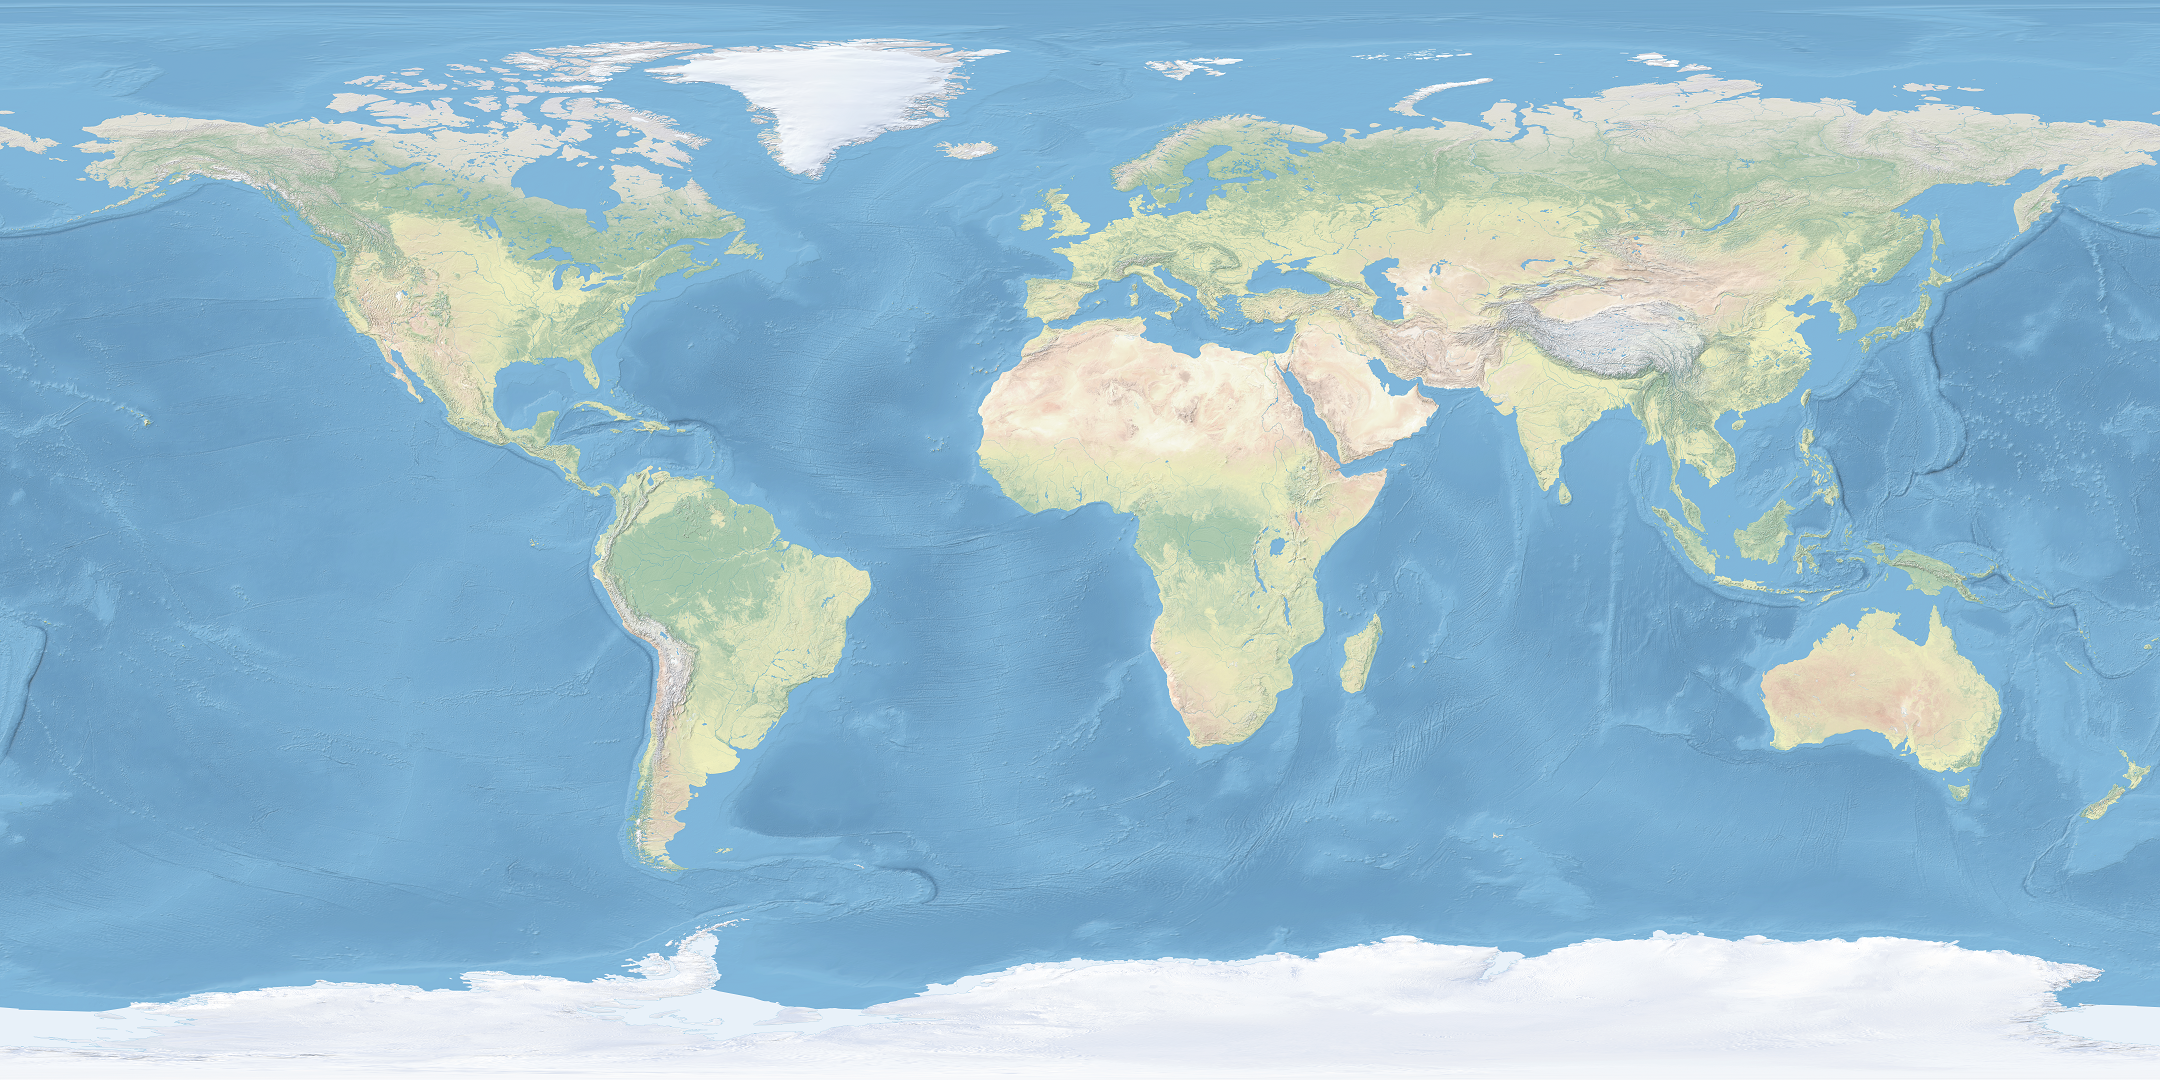
\includegraphics[scale=0.4]{raster_nat_earth.png}
\caption{Rasterbild des Natural-Earth-Datensatzes \protect\footnotemark}
\end{figure}
\footnotetext{http://www.naturalearthdata.com/downloads/10m-raster-data/10m-natural-earth-1/}

\section{Algorithmen in der Geoinformatik}
\section{Verschiedene Arten und ihre Anwendungszwecke}

%----------------------------------------------------------------------------------------
%	CHAPTER 2
%----------------------------------------------------------------------------------------



\chapter{Deep Learning}

\section{Was ist Machine Learning?}
Definition:\newline
Machine Learning ist eine Unterdisziplin der künstlichen Intelligenz und basiert auf der Idee, biologische Denkprozesse, wie sie in Gehirnen ablaufen, nachzuahmen\cite{geofront}.

\textit{A computer program is said to learn from experience E with
respect to some class of tasks T and performance measure P if its performance at tasks in T, as measured by P, improves with experience E.}\cite{michell}

\bigskip

Anders ausgedrückt: Ein Computerprogramm lernt genau dann dazu, wenn es sich hinsitlich seiner Performance in bestimmten Aufgabengebieten mithilfe einer Erfahrung selbständig verbessert.

\section{Motivation und Anwendungsgebiete}
Ziel von Machine Learning in den Geowissenschaften ist es, Muster in Geodaten zu erkennen, Vorhersagen zu machen und Phänomene besser erkennen und verstehen zu können.

\bigskip

Eine Stadt ist ein Komplexes System, das aus vielen kleineren interagierenden Subsystemen besteht. Diese werden durch Faktoren wie Politik, Bevölkerungswachstum, Verkehrsinfrastruktur und den Arbeitsmarkt beeinflusst.
Um zu verstehen, welche Kräfte strukturelle Änderungen von Städten vorantreiben, werden sowohl Satellitenbilder als auch nutzerbezogene Positionsdaten aus sozialen Netzwerken wie Facebook und Twitter und Attributierte Markierungen auf Geoinformationssystemen wie OpenStreetMap\footnote{https://www.openstreetmap.org} verwendet, um Langzeitvorhersagen zur erstellen.
Außerdem helfen diese Modelle und Simulationen dabei, die Mechanismen der urbanen Evolution zu erforschen und Städteplanung zu optimieren.

\bigskip

Im Folgenden eine Auflistung verschiedener Probleme, für deren Lösung sich die Anwendung eines Neuronalen Netzwerks eignet:

\begin{itemize}
\item Klassifizierung - Was ist auf einem Bild zu sehen?
\item Lokalisation - Wo ist das Objekt auf dem Bild?
\item Segmentierung - Klassifizierung jedes Pixels
\item Lineare Regression - Lässt sich ein funktionaler Zusammenhang zwischen den Daten des Datensatzes finden, welcher eine Vorhersage zum weiteren Verlauf der Daten ermöglicht?
\item Clustering - Wie lassen sich Daten vergleichen und in Gruppierungen bei gewisser Ähnlichkeit Ihrer Attribute zusammenfassen?
\item Image Captioning - Wie lassen sich die klassifizierten Objekte in Beziehung setzen? 
\end{itemize}

\begin{figure}[h]
\centering
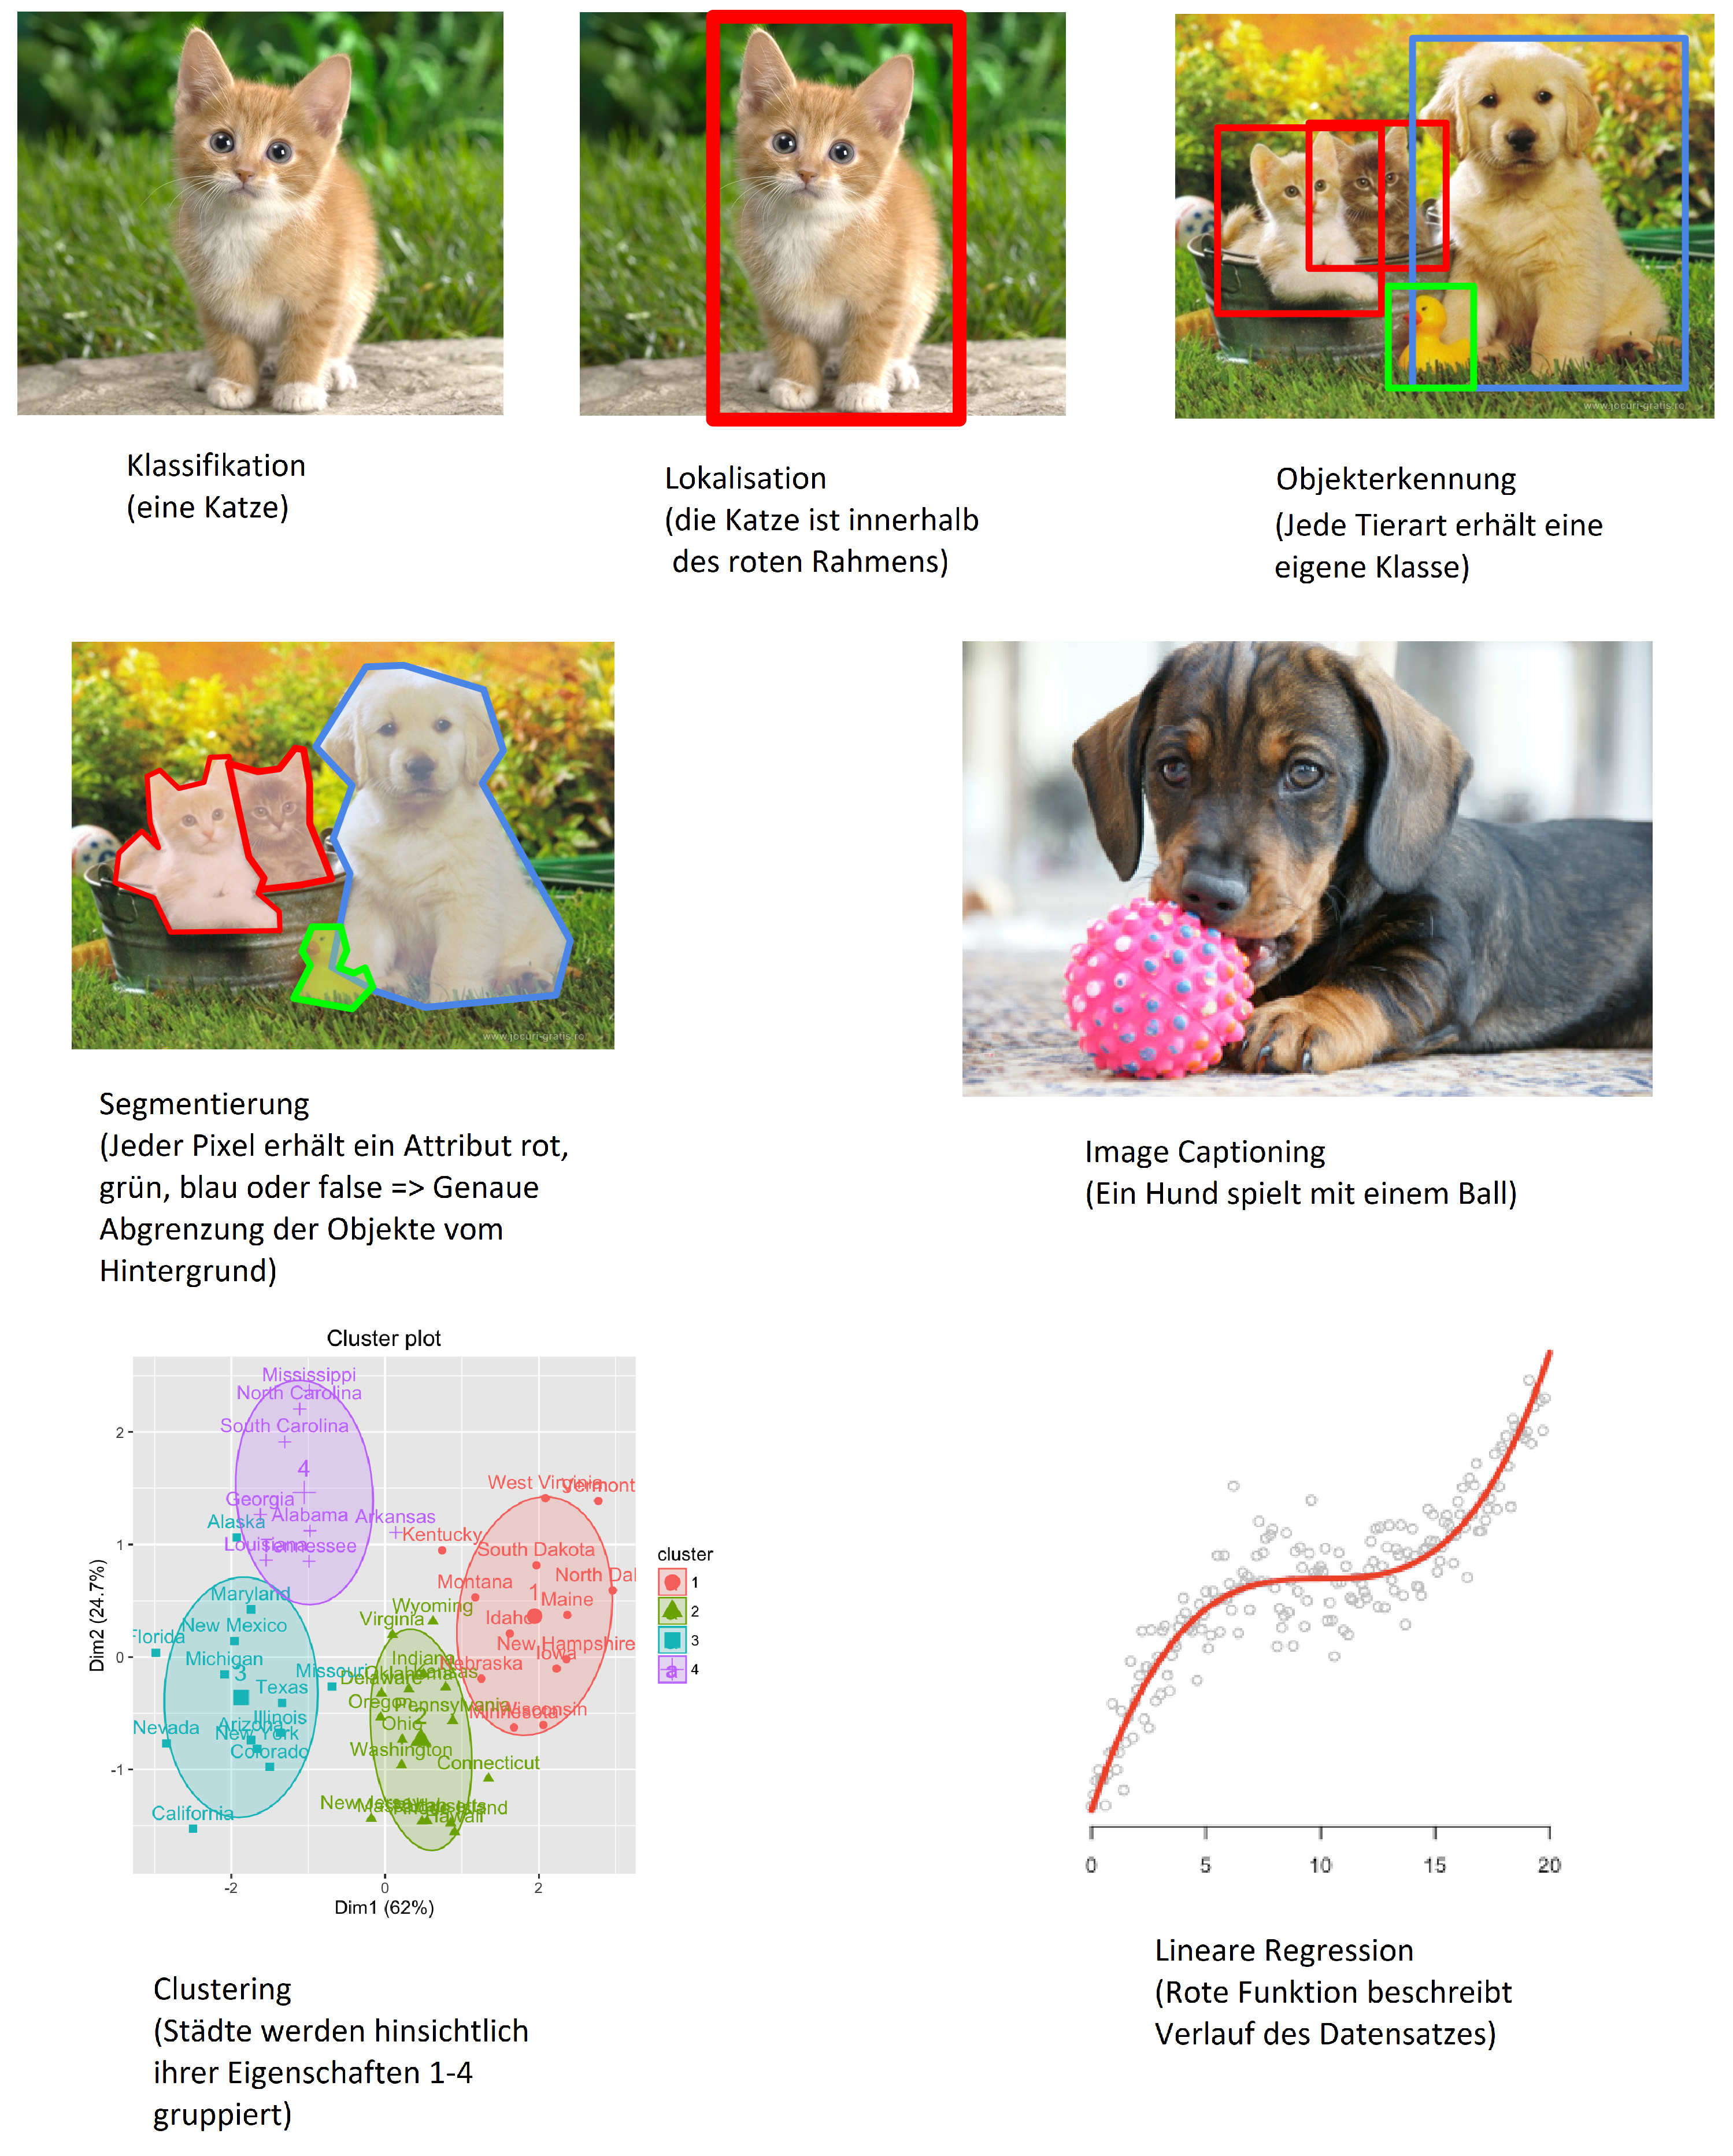
\includegraphics[scale=0.25]{anwendungen.png}
\caption{Vergleich verschiedener Anwendungszwecke von Deep Learning}
\end{figure}


\section{Machine Learning in Geowissenschaften}

\subsection{Herausforderungen und Chancen von Machine Learning}
Die moderne Geowissenschaft steht vor vielen Herausforderungen, wie den Prognosen zu Klimawandel, Luftverschmutzung, Naturkatastrophen, Ressourcenverbrauch, Risiken für Erdbeben, Landrutsch, Vulkanausbrüchen. Die Forschung an solchen Problemen macht die interdisziplinäre Arbeit sämtlicher Wissenschaften unumgänglich.
Geowissenschaften haben sich in den letzten Jahrzehnten von einem data-poor zu einer big-data Disziplin entwickelt. Diese wurde möglich duch die vielen technologischen Verbesserungen wie dem Wachstum der Computerleistung, welche nun große Simulationen ermöglicht und der Demokratisierung von Datenbeständen öffentliche Verbreitung im Internet und einer vielseitigen Beteiligungsmöglichkeit (crowd-source). Die wachsende Verbreitung großer geowissenschaftlicher Datenbestände ermöglicht ein enormes Potenzial für Maschinelles Lernen.

Physikalische Gesetze beschreiben häufig Objekte mit amorphen Grenzen und zwischenbeziehungen. ...knowledge discovery und data mining

Die Erde ist ein komplexes dynamisches System bestehend aus Litosphäre, Biosphäre, Atmosphäre, Hydrosphäre. Einzelne Bestandteile dieses Systems (z.B. Ozeanschichten oder die Bodenbedeckung) befinden sich in einem ständigen Wandel und interagieren miteinander über Prozesse wie Regen oder Magmaeruptionen. Um an Daten solcher Phänomene heran zu kommen, gibt es zwei Möglichkeiten:
\begin{itemize}
\item Messen mithilfe von Sensoren in/auf Satelliten, Flugzeugen, Ballons, Drohnen, Wetterstationen, Schiffen, Boyen.\newline
Sensorbasierte geowissenschaftliche Beobachtungen sind nicht uniform gerastert und beziehen sich häufig auf irreguläre Zeitintervalle (zum Beispiel schwankt die Position einer Boye mit der Zeit). Sie eignen sich jedoch Hervorragend zum sammeln von Daten wie Oberflächentemperatur, Luftfeuchtigkeit, Optische Reflektion, Chemische Zusammensetzung der Atmosphäre, Strömungen und Drücke, Emissionen, seismische Aktivität und die Oberflächengestalt der Erde. Diese Vielfalt an geologischen Eigenschaften erfordert bezüglich eines gegebenen Problems eine individuelle Zusammenstellung von relevanten Datensätzen. Die Datentypen müssen gegebenenfalls konvertiert und die Datenbestände interpoliert werden, um sie besser interpretierbar zu machen.

\item Ableiten aus mathematischen Modellen und Simulationen
Geologische Prozesse, ihre Interaktionen und Änderungen sind auf physikalische Gesetze zurückzuführen. Zum Beispiel sind Bewegungen von Wasser in der Liosphäre auf die Strömungsdynamic zurückzuführen. Ein Nachteil physikalischer Berechnungen auf Grundlage von Modellen für komplexe Systeme ist leider deren Ungenauigkeit. Dennoch eignen sie sich zur näherungsweisen Darstellung des zeitlichen Verlaufes von geophysikalischen Phänomenen. Ein weiterer Vorteil ist, dass Simulationen besonders große Datensätze erzeugen können, wenn Daten für große Zeitintervalle von Interesse sind. Diese ermöglichen dann wiederum eine Datenbasierte Analyse mittels Machine Learning.
\end{itemize}

Herausforderungen: Leider ist die Nützlichkeit von Machine Learning für Knowledge Discovery häufig begrenzt. Geophysikalische Objekte sind häufig nicht klar definiert (keine klar definierten Grenzen) und ändern sich häufig. Daten zu solchen Objekten können ebenfalls unterschiedliche Auflösungen haben, rauschen, unvollständig oder ungenau sein. Auch kann die zeitliche Auflösung aus historischen Gründen stark variieren (z.B. ein Weltkrieg, in dem historische Datensätze zerstört wurden). Auch liegen häufig nicht ausreichend Geländedaten vor. Die Herausforderungen lassen sich in 3 Hauptkategorien unterteilen:

\begin{itemize}
\item \textbf{Eigenschaften Geologischer Prozesse}
\begin{itemize}\item Amorphe Grenzen (Wellen, Flüsse, Stürme) - Segmentierungs- und Clusteringverfahren sowie Maßnahmen für Feature-Charakterisierungen sind notwendig.
\item Raumzeitliche Struktur - 
Für viele Machine Learning Methoden nimmt man an, dass beobachtete geophysikalische Eigenschaften nicht korrelieren und die erhobenen Daten gleichverteilt sind. Die Realität sieht anders aus: 
Benachbarte Orte sind stark korreliert (Wahrscheinlichkeit für Grasland ist in der Nähe eines Waldes größer als in einer Wüste). Änderungen (Wald => Wüste) bewirken Zustände, die für eine unbestimmbare Zeit persistieren (Die Wüste wird nicht regelmäßig zum Wald und umgekehrt), was auf Klimaveränderungen zurückzuführen ist.
Zwei weit entfernte Orte können ebenfalls stark korrelierte Eigenschaften besitzen (z.B. Temperatur, Druck). Man nennt diese meist meteorologischen Korrelationen Telekonnektionen .
\item Hochdimensionalität - Die Erde ist eines der komplexesten bekannten Systeme mit einer extrem großen Anzahl an Variablen, die alle miteinander in sowohl räumlich als auch zeitlich relativ zur Größe der Erde winzigen Skalen miteinander wechselwirken. Für solche Verarbeitung und Speicherung von Daten solcher Systeme ist die Rechenleistung heutiger Computer nicht ausreichend.
\item Raumzeitliche Variabilität - Geologische Prozesse können stark schwanken, sowohl in kurzen Zeitintervallen (Jahreszeiten, Tidenhub), als auch in langen Zeitintervallen (Polsprung, Präzession, Klimawandel) als auch räumlich (Gebirgsformationen, Vegetationszonen, Klimazonen) => Es ist sehr schwierig ein Modell zu trainieren, dass alle diese Prozesse vereint. Eine lokale und zeitliche Begrenzung der Datensätze ist zwingend erforderlich.
\item Seletene Phänomene - Seltene Ereignisse wie z.B. Vulkanausbrüche, Tsunamis und Erdbeeben verfälschen das Modell, da sie nur für ein Training auf viel größeren Zeitskalen geeignet sind. Aus diesem Grund müssen sie erkannt und aus dem Modell  herausgerechnet werden. Dies ist nahezu unmöglich, da es für solche Ereignisse keine ausreichenden Erfahrungswerte gibt.
\end{itemize}

\item \textbf{Sammeln von Geodaten}
\begin{itemize}
\item Daten mit verschiedenen Auflösungen - Beispiel: Zur Beurteilung von Waldbränden müssen Bilder aus Luftaufnahmen und Satellitenbilder miteinander kombiniert werden. Die Flugzeugbilder haben eine höhere räumliche Auflösung, die Satellitenbilder wurden jedoch in regelmäßigen Zeitabständen aufgenommen. Aus diesem Grund müssen Interpolations- oder Upsamplingmethoden entworfen werden, um die beiden Arten von Bildern vergleichbar zu machen.
\item Rauschen, Unvollständigkeit, Ungenauigkeit - Viele Geodatensätze sind unvollständig oder rauschen, weil z.B. Sensoren temporär ausgefallen sind oder unter verschiedenen Wetterbedingungen Messungen durchgeführt haben. Manche Daten sind erst dann interpretierbar, wenn Sie mit einem mathematischen Modell kombiniert werden. Dieses kann die Interpretierbarkeit jedoch ebenfalls beeinflussen.
\end{itemize}

\item \textbf{Mangelhafte Datensätze}
\begin{itemize}
\item Kleine Sample-Größe - Viele Datenbestände sind niedrigfrequent und extrem ungenau, wenn sie aus einer Zeit stammen, in welcher es entweder keine oder nur wenige Messinstrumente gab. Auch gibt es Orte, an denen es nur schwer möglich ist (zeitlich hochfrequente) Messungen durchzuführen (Bohrkernanalyse in Antarktis o.ä., Bäume mit ausreichendem Alter für Jahresringe). Eisbohrkerne aus der Antarktis lassen zudem keine Rückschlüsse über die Klimatischen Verhältnisse in anderen Gegenden zu. 
\item Mangelhafte gelabelte Geländedaten - Oft liegen Geländedaten in mangelnder Qualität vor. Dies liegt daran, dass sie nur mit Zeit- und Kostenintensiven Maßnahmen zu beschaffen sind. Eine mangelhafte Datenqualität führt zu einem langsamen Trainingsprozesses und zu Unter oder Überanpassung des Modells, was die Aussagekraft stark einschränkt.
\item Aus beiden oben genannten Gründen müssen Trainingsmodelle entwickelt werden, die mit kleineren Datensätzen zurecht kommen.
\end{itemize}
\end{itemize}


\subsection{Beispiele}

\section{Tensorflow}
\section{Erstes eigenes CNN}

%----------------------------------------------------------------------------------------
%	CHAPTER 3
%----------------------------------------------------------------------------------------

\chapter{Clusteringverfahren}
\section{Probabilistisches und Possibilistisches Clustering}
\subsection{FCM und PFCM}
\subsection{Vorraussetzungen für die Anwendung auf Geodaten}
\subsection{Eigener Algoritmus (noch ohne Name)}
\section{CVI}
\subsection{NPC}
\subsection{FHV}
\subsection{Otsu-Binarisierung}
\subsection{VAT-Algorithmus}
\section{Clustering auf unvollständigen Daten}

%----------------------------------------------------------------------------------------
%	CHAPTER 4
%----------------------------------------------------------------------------------------

\chapter{Fazit und Ausblick}
\section{Ausblick - Mein Thema für die Masterarbeit}

\printbibliography

\vfill
\end{document}